\scanpage{31}
du repère (défini par $\pi,\tau,\Omega$) définit un ordre sur $T$, car $\pi$ définit une structure pentagonale, $t_0=\tau$ une origine pour celle-ci, et désignant par $t_1=u$ l'unique $\in\Omega$ adjacent à $\tau$, on trouve un repère de \deleted{\unsure{$\mathscr P_2$}} $(T,\pi)$, d'où une énumération $T=\{t_0,t_1,t_2,t_3,t_4\}$, \inserted{qui est compatible avec l'orientation $\unsure{\bar\omega|\varpi}$.} Inversement, la donnée d'une telle énumération définit une structure pentagonale $\pi\in\mathrm{Pent}^{\unsure{+|2}}(T,\bar\omega)$, \deleted{un $\Omega=\{t_1,$} un $\tau=t_0\in T$, un $\Omega=\{t_1,t_3\}\in\unsure{\mathscr P|\mathfrak P}_2(T)$, définissant un élément de $\mathrm{Rep}(\bar\Pi)$ \ldots.

\figure{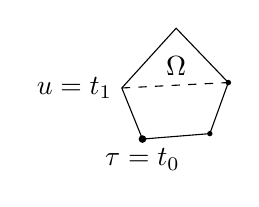
\begin{tikzpicture}[scale=.69]
\coordinate(u)at(-1,0);\coordinate(b)at(0,1.1);\coordinate(c)at(.96,.1);
\coordinate(d)at(.62,-.84);\coordinate(t)at(-.62,-.94);
\draw(u)--(b)--(c)--(d)--(t)--cycle;\draw[dashed](u)--(c);
\fill(t)circle(2pt) (c)circle(1.45pt) (d)circle(1.4pt);\node[left]at(u){$u=t_1$};\node[above]at(0,.05){$\Omega$};
\node[below]at(t){$\tau=t_0$};
\end{tikzpicture}}

Il reste à expliciter [pour $\Pi$ orienté]
\[
\left\{\begin{aligned}
\widetilde{S}(\bar\Pi)&\simeq S(\Pi)\\
\widetilde A(\bar\Pi)&\simeq A(\Pi)\\
\widetilde F(\bar\Pi)&\simeq F(\Pi)
\end{aligned}\right.
\]
en termes de $(T,\bar\omega)$. Et expliciter aussi, \deleted{\unsure{tant}} qu'à faire, la structure de $\bar\Pi$ comme polyèdre quotient \ldots.
% archive sheet number: 30
